\documentclass{article}
\usepackage[a4paper,margin=1in]{geometry}
\usepackage{amsmath}
\usepackage{graphicx}
\usepackage[colorlinks=true, allcolors=blue]{hyperref}
\usepackage{tikz}
\usepackage{gensymb}
\usepackage{float}



\title{IB2\\
Verslag 1}
\date{11/10/2023}
\author{Tom Thys, Daan Vercammen, Sander Haustraete}

\begin{document}
\maketitle

\begin{minipage}{\textwidth}
    \centering
    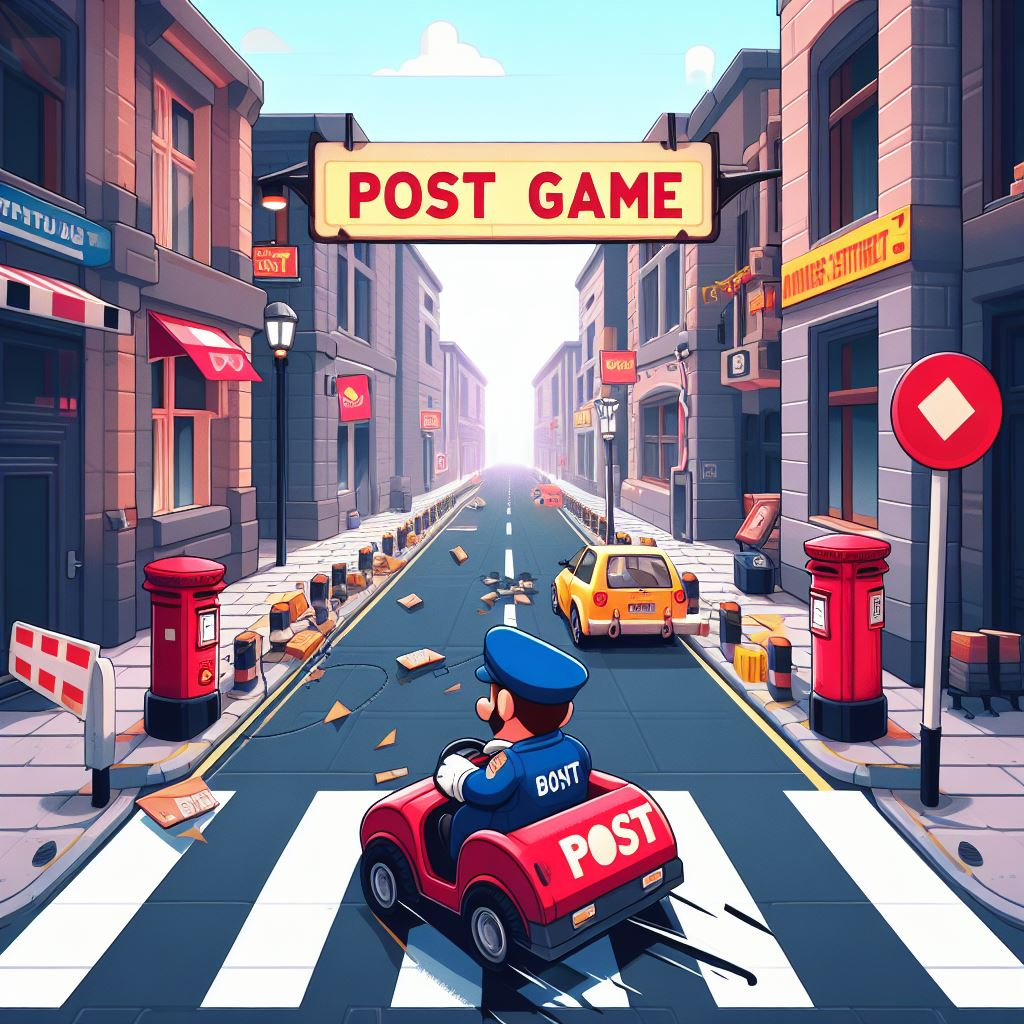
\includegraphics[width=0.7\textwidth]{fotos/_a1a1db80-3fb5-41c9-9da6-cb8f494513cb.jpg}
\end{minipage}

\vspace{50pt}

\begin{minipage}{\textwidth}
    \centering
    
\includegraphics[width=0.5\textwidth]{fotos/Logo.png}

\end{minipage}

\newpage
\pagenumbering{arabic}

\section{Scope of the application}
\subsection{Doel}
Het doel van het spel is vrij simpel, breng als postbode in 1 minuut zoveel mogelijk pakjes naar de juiste plaats. Dit doe je 
door rond te rijden in een lange straat. Op je scherm zie je een gps die je de juiste richting aangeeft. Wanneer je op het juiste adres
bent, komt op je gps je nieuwe locatie. Maar het is natuurlijk niet gewoon van punt a naar punt b rijden. De straat staat namelijk
vol met obstakels zoals bomen en vuilnisbakken. En er rijden natuurlijk ook andere auto's rond in de straat. Wanneer je tegen een van 
die obstakels of andere auto's botst ben je verloren... 
\subsection{Doelgroep}

\section{overview and features}
\subsection{Extra's}


\end{document}